\documentclass[specialist, subf, href, colorlinks=true, 14pt, final]{disser}
\usepackage[a4paper, mag=1000, includefoot, left=3cm, right=1.5cm, top=2cm, bottom=2cm, headsep=1cm, footskip=1cm]{geometry}

\usepackage[T2A]{fontenc}
\usepackage [utf8] {inputenc}
\usepackage[english, russian]{babel}
\usepackage{caption}
\usepackage{enumerate}
\usepackage{amsmath,amsthm,amssymb}
\usepackage{wrapfig}
%\usepackage {enumitem}  
%\usepackage{graphicx}
%\usepackage{multicol}
\usepackage{mathrsfs}
\usepackage{xcolor}
\usepackage{tikz}
\usetikzlibrary{decorations.pathreplacing}
\setcounter{tocdepth}{2}
%\usepackage{hyperref}
%\usepackage{algorithm}
%\usepackage[noend]{algpseudocode}
%\usepackage[margin=1in]{geometry}

\theoremstyle{definition}
\newtheorem{defn}{Определение}[section]
\newtheorem{example}{Пример}[section]
\newtheorem{state}{Утверждение}[section]
\newtheorem{theorem}{Теорема}[section]
\newtheorem{lemma}{Лемма}[section]
\newtheorem{axiom}{Аксиома}[section]
\newtheorem{consequence}{Следствие}[section]

\newcommand{\anonsection}[1]{\section*{#1}\addcontentsline{toc}{section}{#1}}
\newcommand{\anonsubsection}[1]{\subsection*{#1}\addcontentsline{toc}{subsection}{#1}}
\newcommand{\pdfrac}[2]{\frac{\partial #1}{\partial #2}}
  
 % Цвета для гиперссылок
\hypersetup{pdfstartview=FitH, linkcolor=blue, urlcolor=blue, colorlinks=true}


\begin{document}

\begin{titlepage}
\begin{center}
МОСКОВСКИЙ ГОСУДАРСТВЕННЫЙ УНИВЕРСИТЕТ\\
имени М. В. Ломоносова\\
Механико-математический факультет\\
\vspace{1cm}
\begin{figure}[!htp]%
  \begin{center}%
        {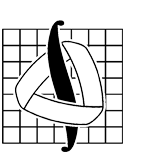
\includegraphics[width=20mm]{pics/mmlogo.png}}%
  \end{center}
\end{figure}
\vspace{4cm}
\Large{
ЗАДАЧИ ФИЗИКО-МЕХАНИЧЕСКОГО ПРАКТИКУМА ПО ГАЗОВОЙ И ВОЛНОВОЙ ДИНАМИКЕ
}\\
\vspace{4cm}
\end{center}
\end{titlepage}

\tableofcontents

\anonsection{Раздел 1}
\anonsubsection{Задача 1. Продольное соударение упругих стержней}
Целью работы является изучение процесса соударения двух стержней и определение скорости упругой волны и деформации, возникающей в стержнях при ударе.\\
I. \underline{Описание явления}\\
Процесс распространения малых возмущений в изотропной 
упругой среде в общем случае можно изучать, исследуя решения 
уравнений Ляме для конкретных начальных и граничных условий [I]. 
Однако общая задача о распространении волн в ограниченном упругом
пространстве довольно сложна. Сен-Венаном разработана 
приближенная теория продольных волн в длинных тонких стержнях. При этом в
качестве основного предположения принята гипотеза плоских 
сечений, т.е. полагается, что любое плоское сечение, образованное
точками среды и перпендикулярное оси стержня, остается при 
движении плоским и перпендикулярным оси, а напряжение во всех 
точках такого сечения одинаково и меняется только со временем. 
Принятые предположения позволяют рассматривать продольное движение
стержней в одномерной постановке.\\
II. \underline{Теоретическая часть}\\
Рассмотрим соударение двух стержней с равной начальной 
длиной $l_0$ , изготовленных из одного и того же материала и имеющих
одинаковое начальное поперечное сечение $S_0$ (Рис. \ref{1-1-1}).
Пусть недеформированный стержень I движется вдоль своей оси
со скоростью $v_0$ и в момент $t = 0$ касается соосного с ним 
стержня II. Для изучения последующего процесса соударения введем 
неподвижную ось $Ox$ с началом, совпадающим с левым торцом первого
стержня в момент $t = 0$.\\
\begin{figure}[!htp]
  \center{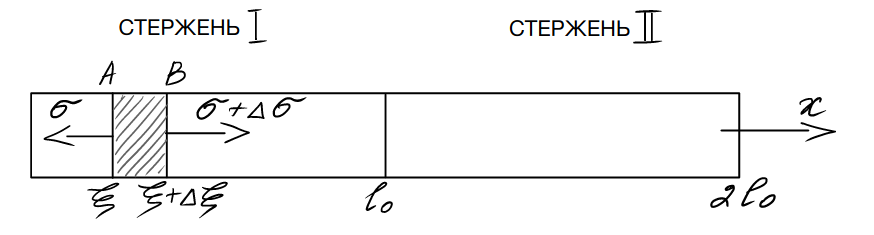
\includegraphics[width=160mm]{pics/1-1-1.png}}
  \caption{}
  \label{1-1-1}
\end{figure}
\\
В качестве лагранжевой координаты рассмотрим начальную 
координату сечения $\xi = x(0)$. Перемещение $u = u(\xi, t)$ можно 
представить в виде
\[
  u(\xi, t) = x(\xi, t) - \xi
\]
Тогда скорость $v$ и продольная деформация $\varepsilon$ в данном сечении $\xi$ соответственно равны
\begin{equation}\label{eq111}
  v = \frac{\partial u}{\partial t},\ \ \varepsilon = \frac{\partial u}{\partial \xi}
\end{equation}
Запишем уравнение движения (второй закон Ньютона) для 
выделенного малого элемента AB (Рис. \ref{1-1-1}), ограниченного сечениями $\xi$ и $\xi + \Delta\xi$:
\begin{equation}\label{eq112}
  \rho\Delta\xi S_{0} \frac{\partial v}{\partial t} = S_{0} \left[\sigma(\xi+\Delta\xi, t) - \sigma(\xi, t)\right],
\end{equation}
где $\rho$ -- начальная плотность материала стержней; $\sigma(\xi,t)$ -- напряжение в данном сечении $\xi$. 
Поделив (\ref{eq112}) на $\Delta\xi$ и сделав предельный переход $(\Delta\xi \rightarrow 0)$, приходим к уравнению
\begin{equation}\label{eq113}
  \rho\frac{\partial v}{\partial t} = \frac{\partial \sigma}{\partial \xi}
\end{equation}
Материал стержней считаем линейно-упругим, т.е.
\begin{equation}\label{eq114}
  \sigma = E\varepsilon,
\end{equation}
где $Е$ - модуль Юнга. 
Уравнения (\ref{eq111}), (\ref{eq113}), (\ref{eq114}) позволяют написать замкнутую систему уравнений для определения скорости и деформации:
\begin{equation}\label{eq115}
  \begin{aligned}
  &\pdfrac{v}{t} = a_{0}^{2} \pdfrac{\varepsilon}{\xi},\\ 
  &\pdfrac{v}{\xi} = \pdfrac{\varepsilon}{t}
  \end{aligned}
\end{equation}
где $a_{0}^{2} = \sqrt{E/\rho}$.
В начальный момент времени $(t = 0)$ первый стержень 
напряжен и имеет скорость $v$, а второй стержень покоится, т.е.
\begin{equation}\label{eq116}
  \begin{aligned}
  &\text{при } t = 0,\ 0 \leqslant \xi < l_{0};\ \varepsilon = 0,\ v = v_{0};\\ 
  &\text{при } t = 0,\ l_{0} < \xi \leqslant 2l_{0};\ \varepsilon = 0,\ v = 0.
  \end{aligned}
\end{equation}
На свободных торцах стержней во всё время движения напряжение равно нулю, поэтому при $t > 0$
\begin{equation}\label{eq117}
  \varepsilon(0, t) = \varepsilon(2l_{0}, t) = 0
\end{equation}
В месте контакта стержней $(\xi = l_{0})$ должны быть равны скорости
и напряжения, т.е. при $t > 0$
\begin{equation}\label{eq118}
  \varepsilon(l_{0}^{-}, t) =\varepsilon(l_{0}^{+}, t),\ \ v(l_{0}^{-}, t) = v(l_{0}^{+}, t)
\end{equation}
Здесь знаки $(-)$, $(+)$ соответствуют значениям функции при подходе слева и справа к точке $\xi = l_0$. Для решения системы (\ref{eq115}) приведем ее к характеристическому виду [\ref{eq112}, \ref{eq113}]. Для этого первое уравнение системы умножим на $dt$, второе -- на $d\xi$ и сложим полученные равенства:
\[
  \pdfrac{v}{t}dt + \pdfrac{v}{\xi}d\xi = a_{0}^{2}\pdfrac{\varepsilon}{\xi}dt + \pdfrac{\varepsilon}{t}d\xi
\]
Левая часть данного уравнения является полным дифференциалом $dv$ для любых $(dt, d\xi)$. Найдем характеристические направления $d\xi = \lambda dt$ такие, вдоль которых и правая часть полученного уравнения является полным дифференциалом. Легко видеть, что таких направлений два $d\xi = \pm a_{0}dt$ в каждой точке фазовой плоскости $(\xi, t)$. \\
Таким образом, мы имеем уравнения характеристик и соотношений на них:
\begin{equation}\label{eq119}
  d\xi = \pm a_{0}dt,\ \ \ dv = \pm a_{0}d\varepsilon
\end{equation}
Полученные соотношения позволяют решить поставленную условиями (\ref{eq116})-(\ref{eq118}) граничную задачу.\\
\begin{figure}[!htp]
  \center{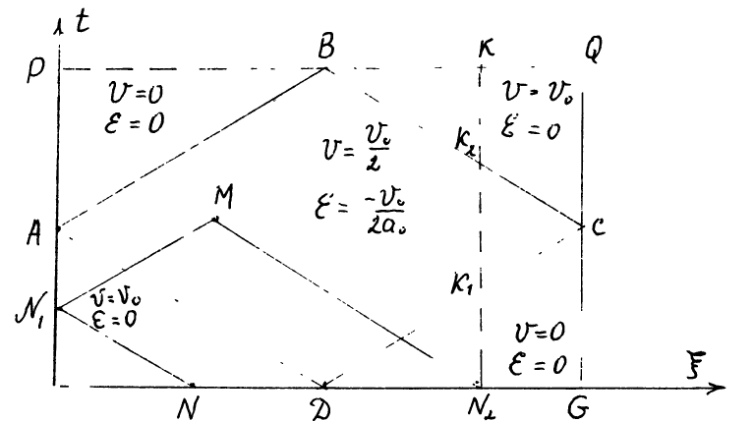
\includegraphics[width=160mm]{pics/1-1-2.png}}
  \caption{}
  \label{1-1-2}
\end{figure}
\\
Покажем это на примере определения решения в точке $M$ (Рис. \ref{1-1-2}). Линии $MN_1$, $MN_2$, $N_{1}N$ являются характеристиками. Сначала определяем решение в граничной точке $N_1$, затем в точке $M$.\\
Из условия (\ref{eq119}) на характеристике $NN_1$ после интегрирования
и использования начальных условий (\ref{eq116}) в точке $N$ получаем $v = -a_{0}\varepsilon + v$. Это уравнение выполняется в любой точке характеристики $NN_1$ и содержит два неизвестных. В точке $N_1$, помимо данного уравнения, должно быть выполнено граничное условие (\ref{eq117}), т.е. в точке $N_1$ мы получили два уравнения для определения скорости и деформации, откуда находим
\begin{equation}\label{eq1110}
  v = v_{0},\ \ \varepsilon = 0.
\end{equation}
Аналогично получаем:
\begin{equation}\label{eq1111}
  \begin{aligned}
  &\text{на характеристике } N_{1}M:\ \ v = a_{0}\varepsilon + v_{0};\\
  &\text{на характеристике } N_{2}M:\ \ v = -a_{0}\varepsilon;
  \end{aligned}
\end{equation}
постоянные интегрирования здесь определены полученным решением в точке $N_1$ (\ref{eq1110}) и начальными условиями (\ref{eq116}) в точке $N_2$ (Рис. \ref{1-1-2}). Из системы (\ref{eq1111}) находим решение в точке $M$: $v = v_{0}/2,\ \varepsilon = -v_{0}/(2a_{0})$. Данный метод решения позволяет определить значения скорости и деформации в любой точке исследуемой области фазовой плоскости. Найденные решения приведены на Рис. \ref{1-1-2}. Область
$OPQG$ разбита характеристиками $AB$, $BC$, $CD$ и $DA$ на пять частей, в каждой из которых решение постоянно. Отметим, что момент времени, соответствующий прямой $PQ$ фазовой плоскости, будет концом соударения,
поскольку в этот момент условия (\ref{eq118}) не выполняются и происходит разлет стержней.\\
Проанализируем полученное решение (Рис. \ref{1-1-2}). В произвольном
сечении $N_{2}K$ второго стержня поведение решения следующее. До 
момента времени, соответствующего точке $K_1$ (момент прихода волны
нагрузки), все параметры сохраняют свои начальные значения. Затем
скачком меняются и остаются постоянными до момента времени, соответствующего точке $K_2$ (момент прихода отраженной от свободного
торца волны разгрузки $CB$). В момент прохождения волны разгрузки параметры решения в данном сечении снова скачком меняются, причем деформация принимает нулевое значение. Данный анализ позволяет сказать, что распространению возмущений в фазовой плоскости соответствуют характеристики. При этом величина $a_0$ является скоростью распространения возмущений но материальным частицам сечений стержня.\\
III. \underline{Экспериментальная часть}\\
Схема экспериментальной установки приведена на Рис. \ref{1-1-3}. 
Плоско-параллельное движение стержней 1 обеспечивается их подвеской на тягах 2. Заданная скорость соударения определяется высотой $h$, с которой сбрасывается стержень
\[
  v_{0} = \sqrt{2gh}
\]
\begin{figure}[!htp]
  \center{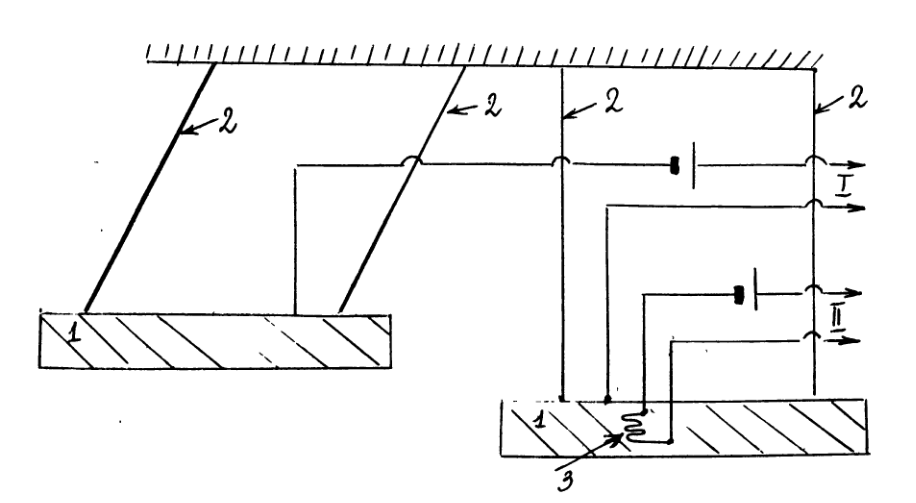
\includegraphics[width=160mm]{pics/1-1-3.png}}
  \caption{}
  \label{1-1-3}
\end{figure}
\\
Эксперимент основан на определении поведения деформации в фиксированном сечении второго стержня, в котором наклеивается тензодатчик 3. В момент касания стержней ($t = 0$) замыкается цепь I запуска развертки осциллографа. На вертикальную развертку осциллографа подается сигнал из цепи II тензодатчика 3. Расстояние от середины тензодатчика до свободного торца второго стержня известно и равно $L$.\\
В результате соударения на экране осциллографа наблюдается сигнал (Рис. \ref{1-1-4}), который фиксируется на фотопленку.\\
\begin{wrapfigure}[7]{l}{0.65\linewidth} 
  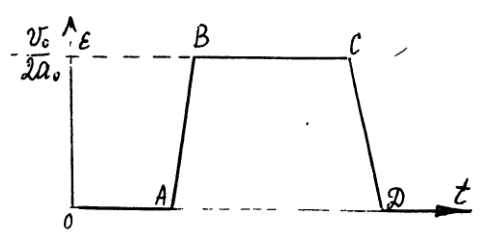
\includegraphics[width=100mm]{pics/1-1-4.png}
  \caption{}
  \label{1-1-4}
\end{wrapfigure}
\\
На Рис. \ref{1-1-4} точка $A$ соответствует времени подхода волны нагрузки к началу тензодатчика, точка $B$ -- времени его полного нагружения. Точки $C$ и $D$ соответствуют началу разгрузки и полной разгрузке датчика отраженной от свободного торца волной. При этом за время $T$, соответствующее длине средней линии трапеции $ABCD$, волна пробегает дважды расстояние $L$ -- от середины датчика до свободного правого торца второго стержня (рис. \ref{1-1-3}). Поэтому экспериментальное значение скорости распространения возмущений 
определяется выражением
\[
  a = \frac{2L}{T}
\]
Высота трапеции $\Omega$ зависит от изменения напряжения в цепи тензодатчика. Изменение напряжения определяется изменением сопротивления датчика в результате его деформации.\\
При линейном усилении сигнала можно считать связь между скачком $\Omega$ и вызывающей этот скачок деформацией линейной, т.е.
\begin{equation}\label{eq1112}
  \varepsilon = k\Omega
\end{equation}
Тензометрический датчик 3 (рис. \ref{1-1-3}) изготовлен из константовой проволоки диаметром 0.03 мм с измерительной базой в 10 мм. Будучи наклеенным на металлический стержень, датчик воспринимает его деформацию. Деформация и изменение сопротивления датчика связаны соотношением
\begin{equation}\label{eq1113}
  \varepsilon = \frac{1}{S}\frac{\Delta R_{g}}{R_{g}}
\end{equation}
где $S$ -- коэффициент тензочувствительности; $R_g$ -- сопротивление недеформированного датчика; $\Delta R_{g}$ -- изменение сопротивления датчика в результате его деформации. Для определения коэффициента пропорциональности $k$ в формуле (\ref{eq1112}) проводится тарировка. Во время тарировки сопротивление в цепи датчика меняется на известную величину путем включения дополнительного сопротивления $R_T$ (рис. \ref{1-1-5}).
\begin{figure}[!htp]
  \center{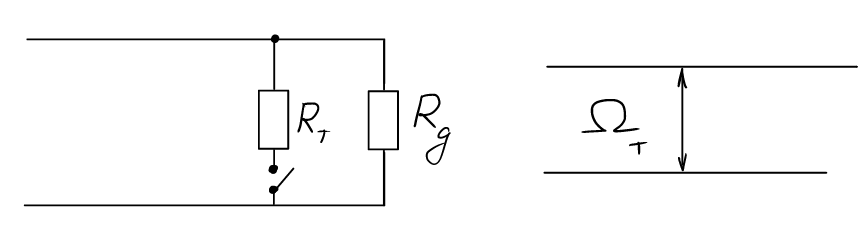
\includegraphics[width=160mm]{pics/1-1-5.png}}
  \caption{}
  \label{1-1-5}
\end{figure}
\\
При включении дополнительного тарировочного сопротивления $R_T$ сопротивление меняется на величину
\begin{equation}\label{eq1114}
  \Delta R_{g} = \frac{R_{g}^{2}}{R_{g} + R_{T}},
\end{equation}
что приводит к скачку $\Omega_{T}$ луча осциллографа. Подставляя изменение сопротивления (\ref{eq1114}) в формулу (\ref{eq1113}), определяем соответствующую данному тарировочному изменению сопротивления деформацию
\[
  \varepsilon_{T} = \frac{R_{g}}{S(R_{g}+R_{T})}
\]
и, учитывая, что $\varepsilon_{T} = k\Omega$, находим из (\ref{eq1112}) экспериментальное
значение деформации
\[
  \varepsilon_{\text{Э}} = \varepsilon_{T}\frac{\Omega}{\Omega_{T}}
\]
\\\\\\
IV. \underline{Порядок выполнения работы}\\
1) В начале работы проводится включение и прогрев осциллографа (согласно инструкции по его эксплуатации). В эксперименте используются два луча. На один из них подается сигнал с датчика, второй луч должен быть установлен на высоте тарировочного скачка первого луча. Поэтому в начале работы проводится включение в цепь датчика тарировочного сопротивления и на высоте подскока первого луча устанавливается второй луч.\\
2) Осциллограф переводится в режим работы с ждущей разверткой лучей и проверяется его автоматический запуск в момент касания стержней.\\
3) Стержень 1 отводится назад, тем самым обеспечивается заданная высота подъема.\\
4) Приводится в готовность фотоаппарат. Фотоаппарат устанавливается на произвольную выдержку.\\
5) Работающий на осциллографе нажимает кнопку фотоаппарата и подает команду на сброс стержня. Фиксация заканчивается после удара.\\
6) Опыт повторяется для других высот подъема стержня.\\
\\
V. \underline{Требования к отчёту}\\
Отчет оформляется и виде заполненной таблицы обработки осциллограмм и проведенных экспериментов и сравнения экспериментальных значений деформации и скорости звука с их теоретическими значениями.
\begin{center}
\begin{tabular}{|c|c|c|c|c|c|c|c|c|c|c|c|}
\hline
N &$h$, мм&$v_0$, м/с&$\Omega$, мм&$\Omega_T$, мм& $\varepsilon_T$ & $\varepsilon_{\text{Э}}$ & $\varepsilon$ & $T$, с & $L$, м & $\frac{\varepsilon_{\text{Э}} - \varepsilon}{\varepsilon}$ & $\frac{a - a_{0}}{a_{0}}$\\
\hline
1 &  &  &  &  &  &  &  & &  &  &\\
\hline
2 &  &  &  &  &  &  &  & &  &  &\\
\hline
\end{tabular}
\end{center}
При этом теоретическое значение деформации определяется решением (рис. \ref{1-1-2}).\\
\\
VI. \underline{Упражнения}\\
1) Определить значение деформации в полубесконечном стержне при его ударе о жесткую преграду, если параметры материала стержня $E, \rho$ известны и известна скорость соударения $v_0$.\\
2) Определить коэффициент тензочувствительности $S$ в формуле (\ref{eq1113}) для датчика, представляющего собой цилиндрическую проволоку длиной $l_0$ и радиусом $r_0$ с известными удельным сопротивлением и коэффициентом Пуассона $\nu$ материала проволоки.\\
3) Определить, пользуясь найденным решением (рис. \ref{1-1-2}), закон движения произвольного сечения.\\
\\
VII. \underline{Контрольные вопросы}\\
1) Какие условия на контактной поверхности возникают при соударении стержней из разных материалов?\\
2) Определить погрешность при определении скорости звука $a$, если считать, что погрешность измерения длины равна 1 мм, а погрешность определения времени $10^{-6}$ с.\\
$L = 144.5$ см; $S = 2.9$ -- коэффициент тензочувствительности;\\
$R_{T} = 3000000$ Ом; $R_{g} = 200$ Ом;\\
$t_{\text{разв}} = 200$ мкс/см; $a_{0} = 5100$ м/с -- теоретическое.\\
\begin{center}
ЛИТЕРАТУРА
\end{center}
1. Седов Л.И. Механика сплошной среды. Т.1,2. М.: Наука, 1970.\\
2. Рахматулин Х.А., Демьянов Ю.А. Прочность при интенсивных кратковременных нагрузках. М.: Физматгиз, 1961.\\
3. Гольдсмит В. Удар. М.: Стройиздат, 1965.\\

\anonsubsection{Задача 2. Сверхзвуковое обтекание клина}
\anonsubsection{Задача 3. Поперечные колебания бруса}
\anonsubsection{Задача 4. Распространение и отражение гидравлического прыжка}
\anonsection{Раздел 2}
\anonsubsection{Задача 1. Волны разгрузки в гибких растяжимых нитях}
\anonsubsection{Задача 2. Изучение процесса разгона поршня в стволе пневматической установки}
\anonsubsection{Задача 3. Нелинейные волны сжатия (растяжения) сдвига в тонкостенной цилиндрической трубе}
\anonsubsection{Задача 4. Прямой экспериментальный метод построения ударных диаграмм сжатия грунтов}
\anonsubsection{Задача 5. Сверхзвуковое обтекание кругового конуса}
\anonsubsection{Задача 6. Соударение двух упругих тел}
\anonsubsection{Задача 7. Экспериментальное исследование подводного взрыва сферического заряда}
\anonsubsection{Задача 8. Влияние вращения цилиндра, находящегося в поперечном потоке, на распределение давления по его поверхности}


\end{document}
